\chapter{Operations and algorithms}

\label{chap:op_al}

Our aim in this chapter is to describe algorithms over 3D data structures. In each description of
algorithm there is a short paragraph that summarizes required operations for running the algorithm.
It is later used in hierarchical implementation of the algorithms.

\section{Converting between representations}

In this section is introduced some algorithms that convert from one representation to another. Each 
representation has it's own capability.

\subsection{Delaunay triangulation}

Let $P$ be a set of points in the $d$-dimensional Euclidean space.
Delanuay triangulation is triangulation such that no point $p \in P$ is inside the circum-hypersphere
of any simplex in $DT(P)$. For better imagination, in case of $2$-dimensional space no point
structure is inside the circumcircle of any triangle of resulting structure.

\subsection{Marching cubes}
\label{sub:march}

Marching cubes algorithm converts from a grid representation to a mesh. It iterates through
all grid elements and build a new polygonial mesh. For an each element (can be considered as \emph{cube}.
In some cases, it can be cuboid or even parallelepiped.)
it determines whether the corners are inside or outside object. The algorithm considers only the elements
those contains both categories of points; rest of them are ignored. As each element has 8 corners,
each of them can be determined either as inside or outside object, in result element can possibly
have one of $2^8 = 256$ configurations. However, some configurations can fit to another after rotation
or reflective simmetry or sign changed case.\\


\begin{figure}[ht]
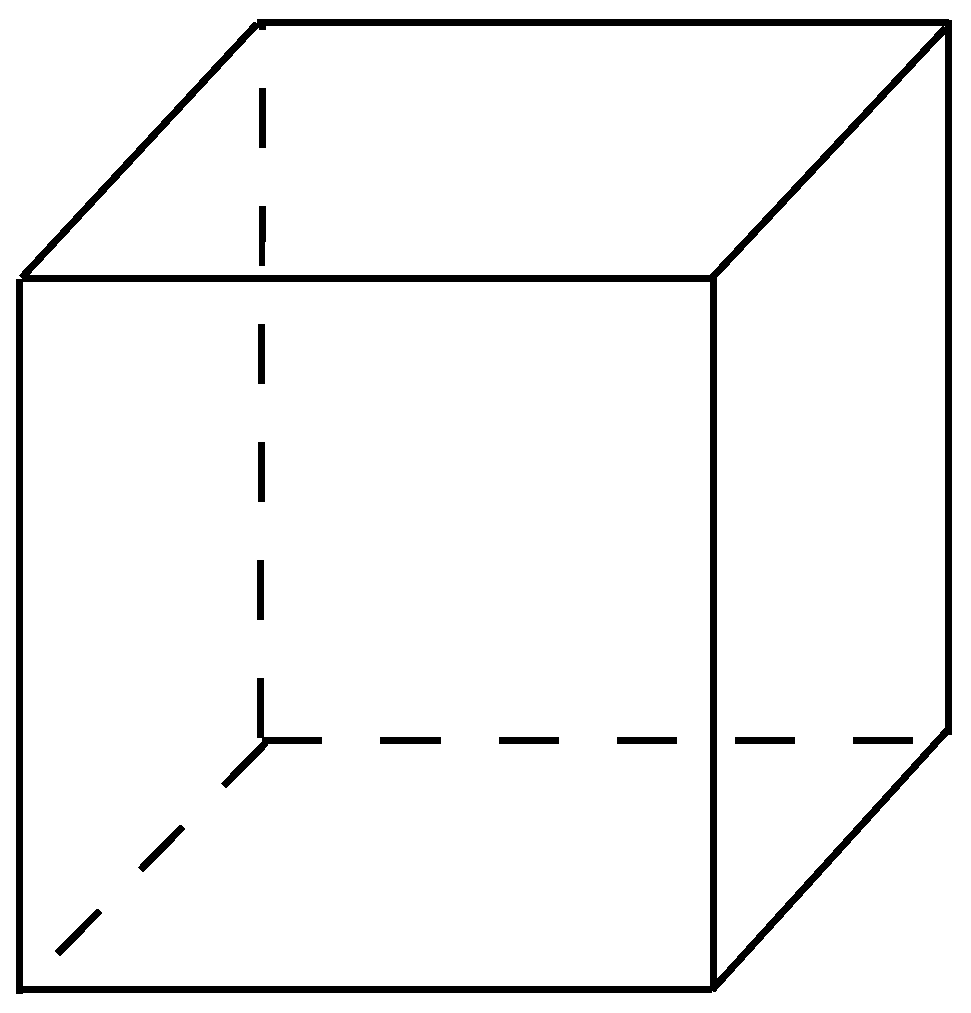
\includegraphics[scale=0.15]{../img/mar_cub_case0.eps}
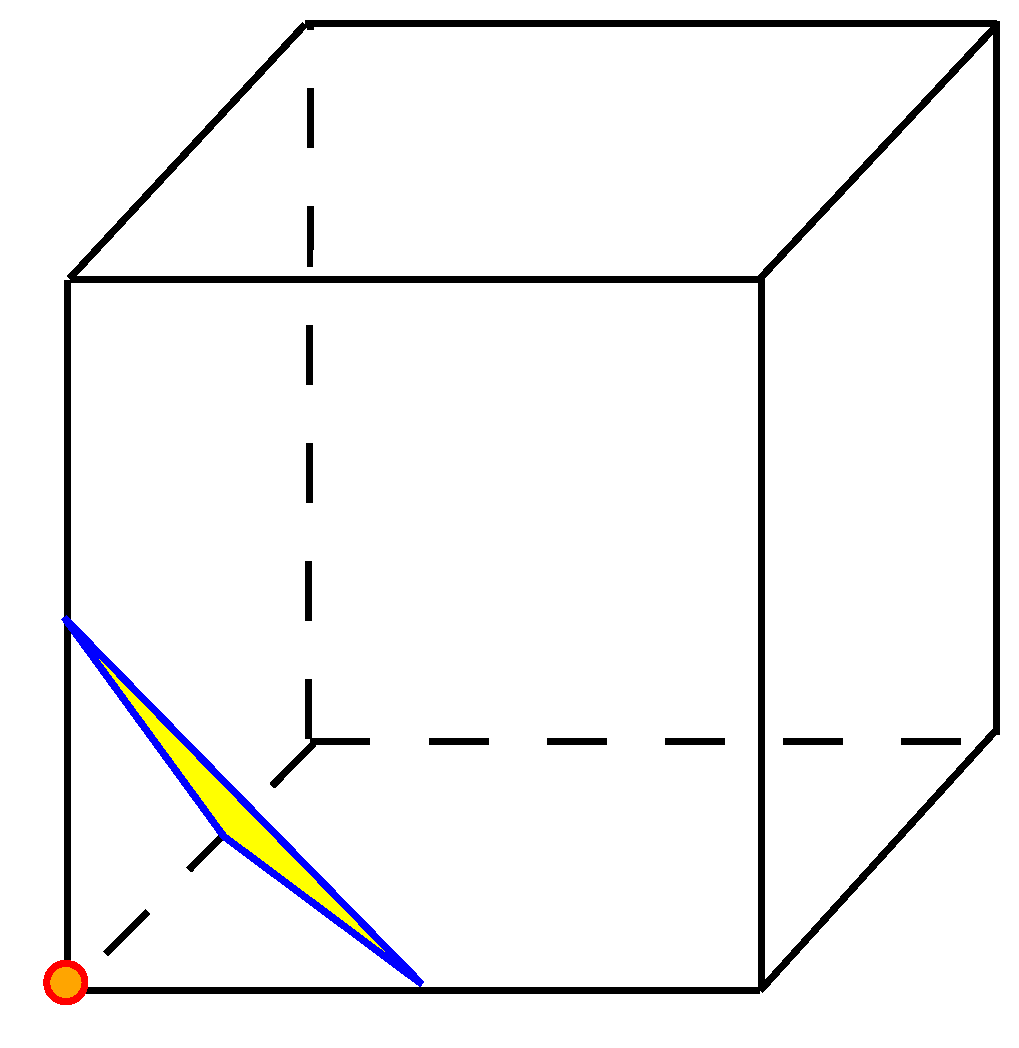
\includegraphics[scale=0.15]{../img/mar_cub_case1.eps}
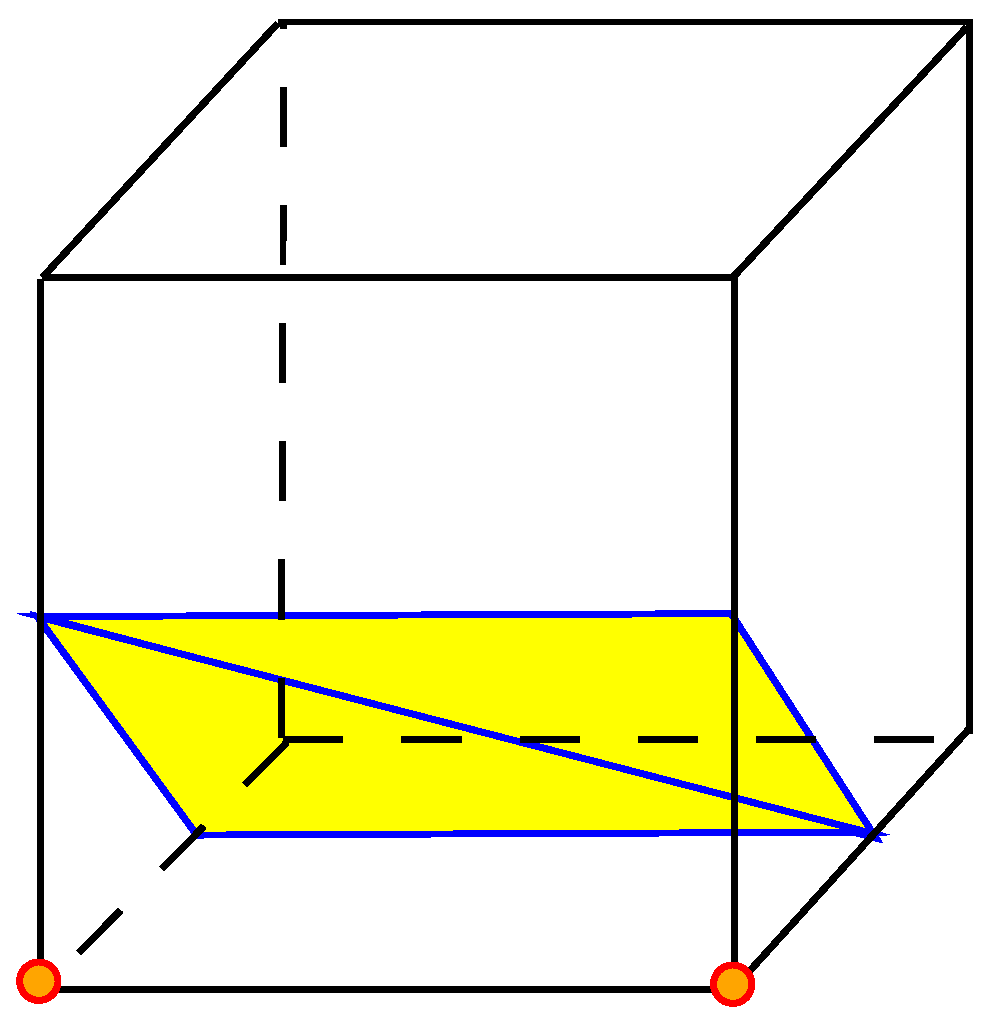
\includegraphics[scale=0.15]{../img/mar_cub_case2.eps}
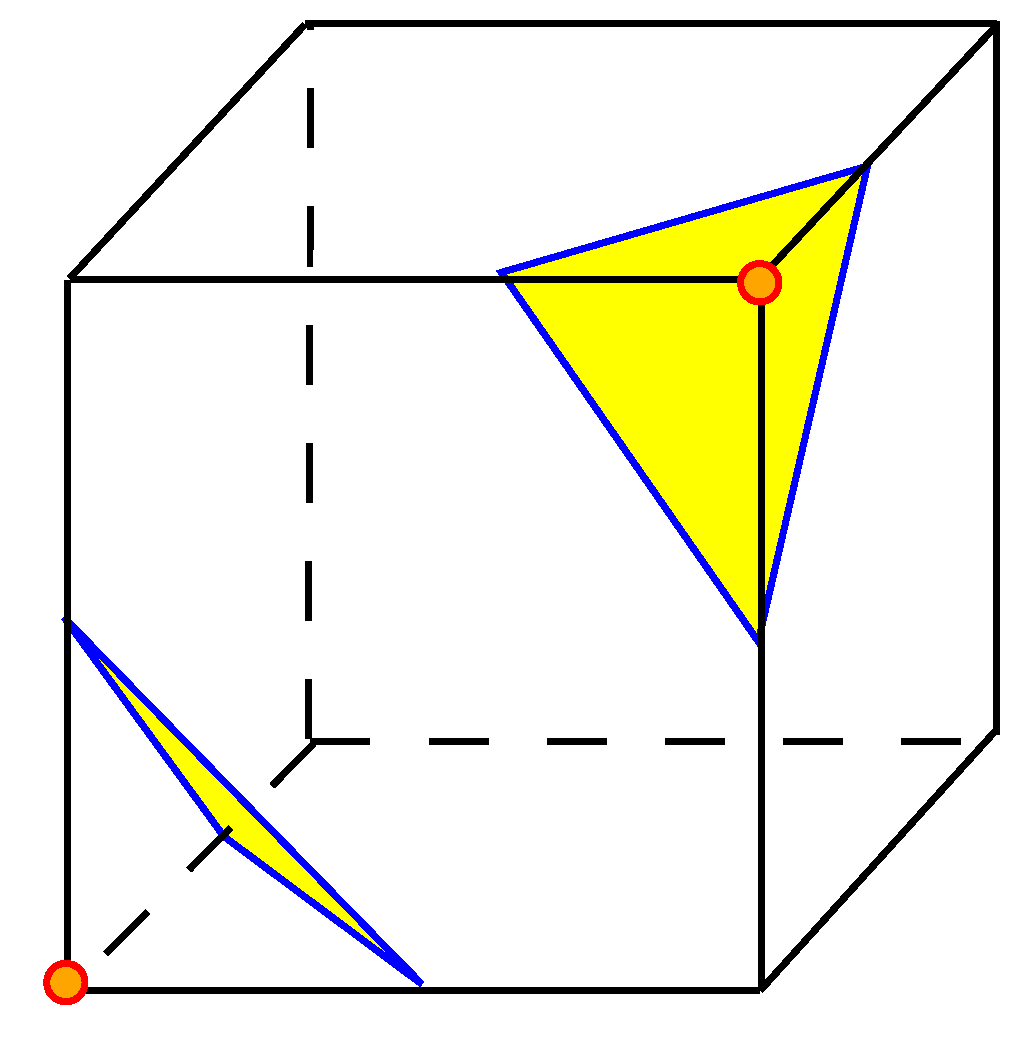
\includegraphics[scale=0.15]{../img/mar_cub_case3.eps}
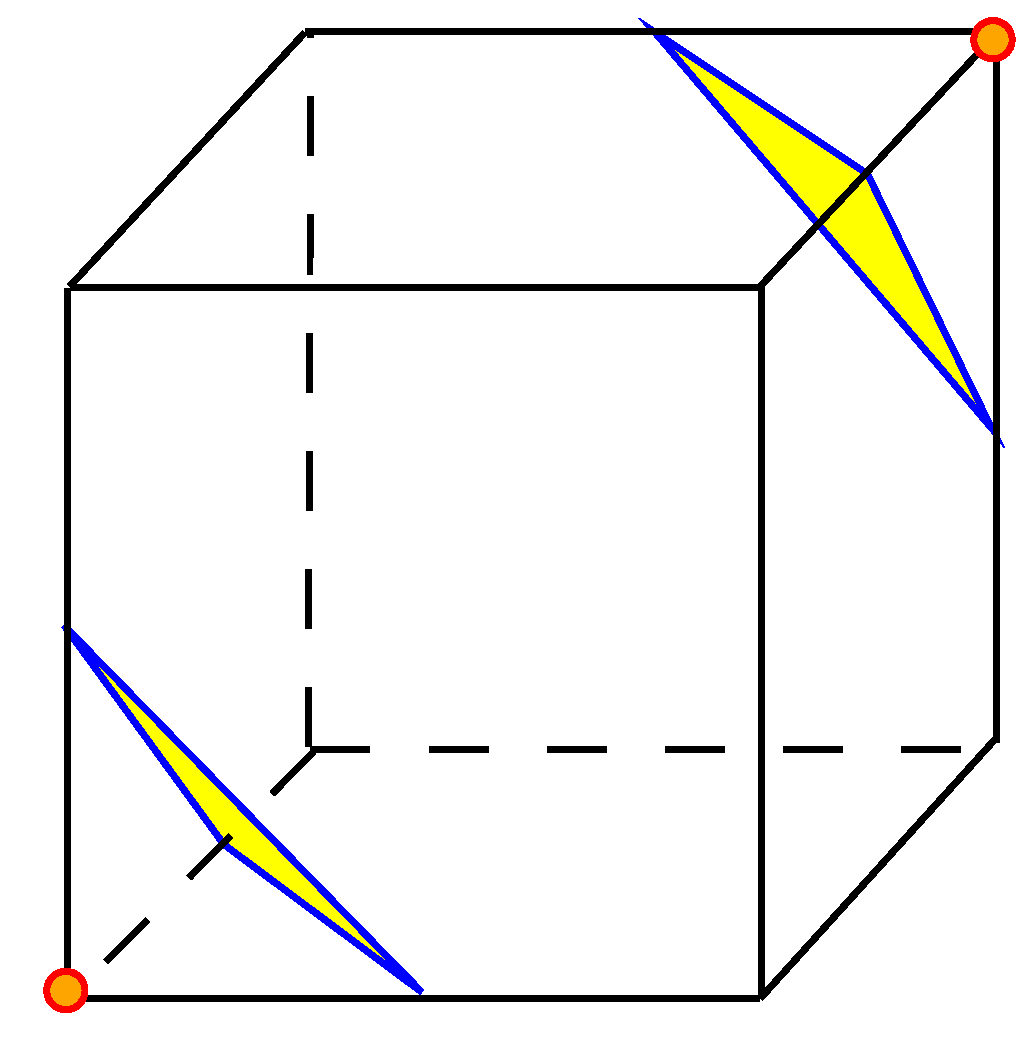
\includegraphics[scale=0.15]{../img/mar_cub_case4.eps}
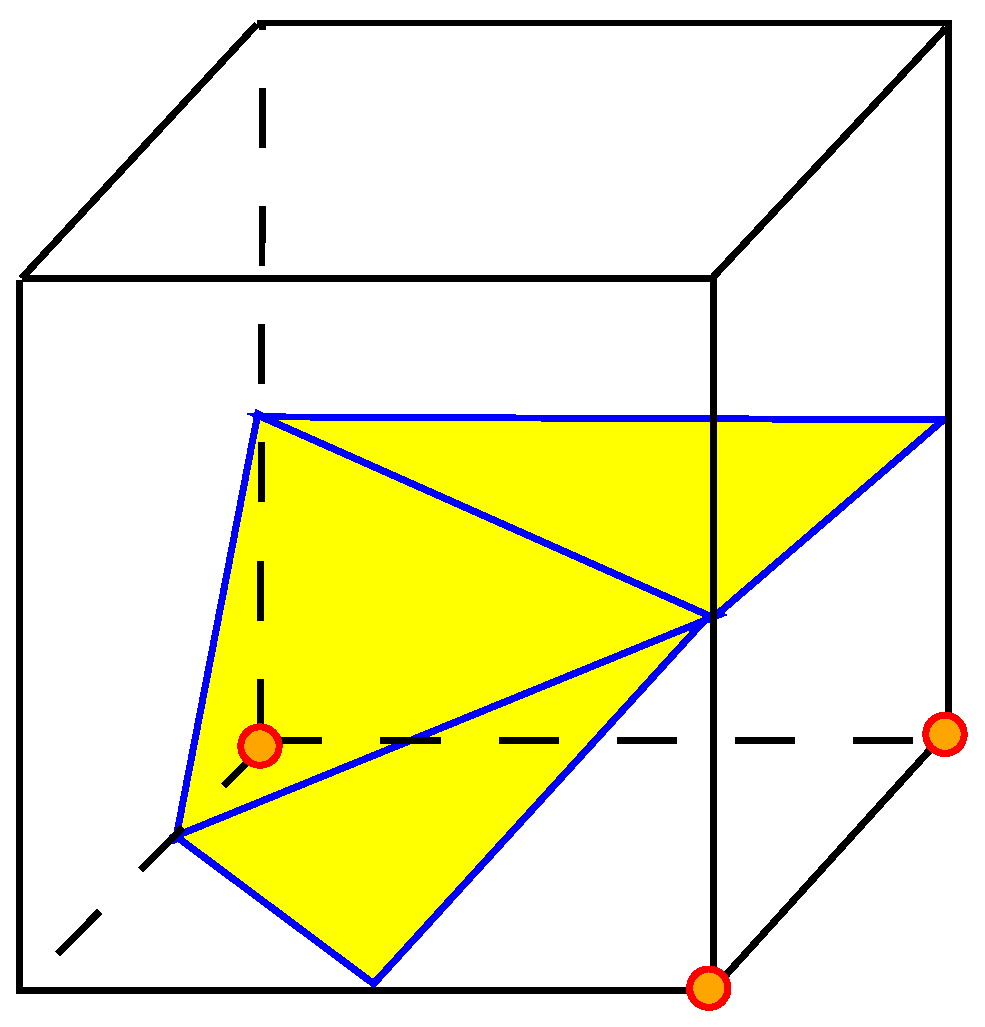
\includegraphics[scale=0.15]{../img/mar_cub_case5.eps}
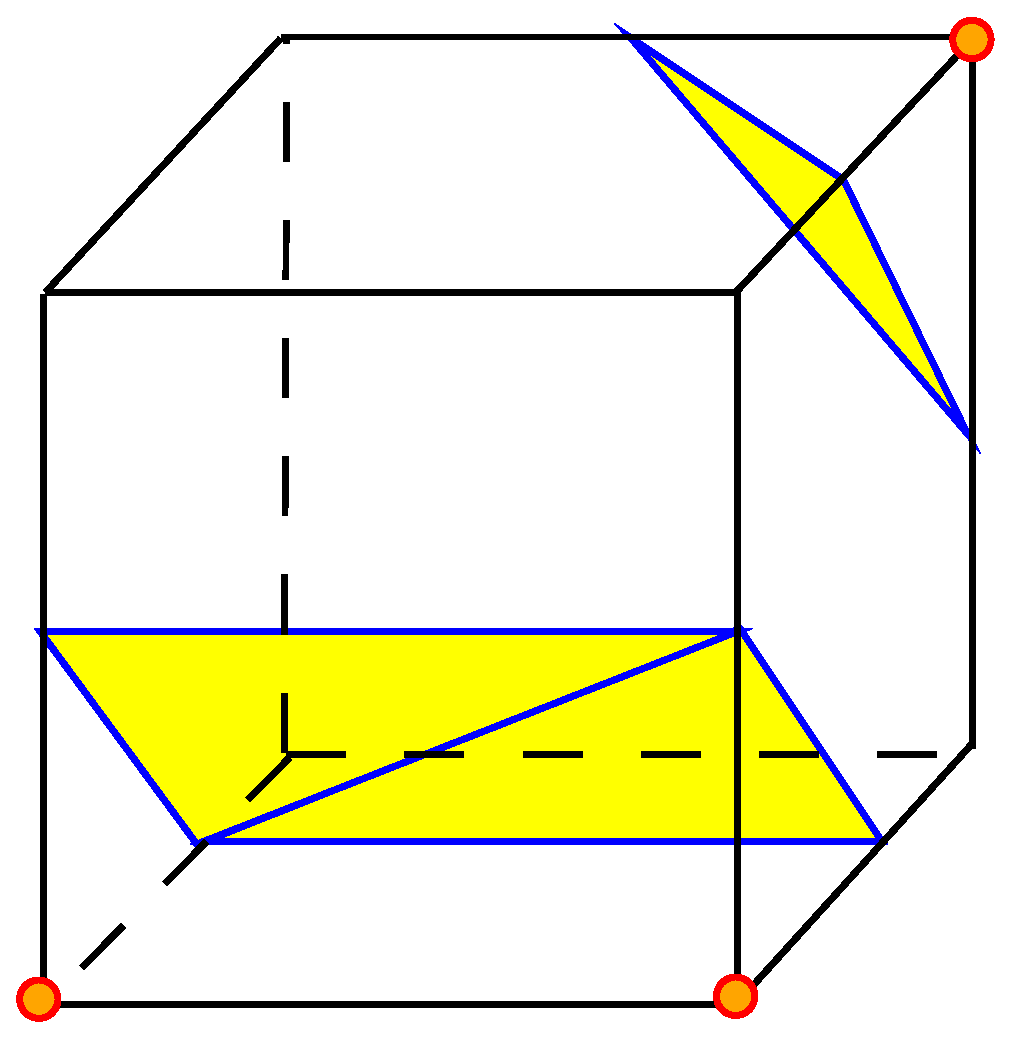
\includegraphics[scale=0.15]{../img/mar_cub_case6.eps}
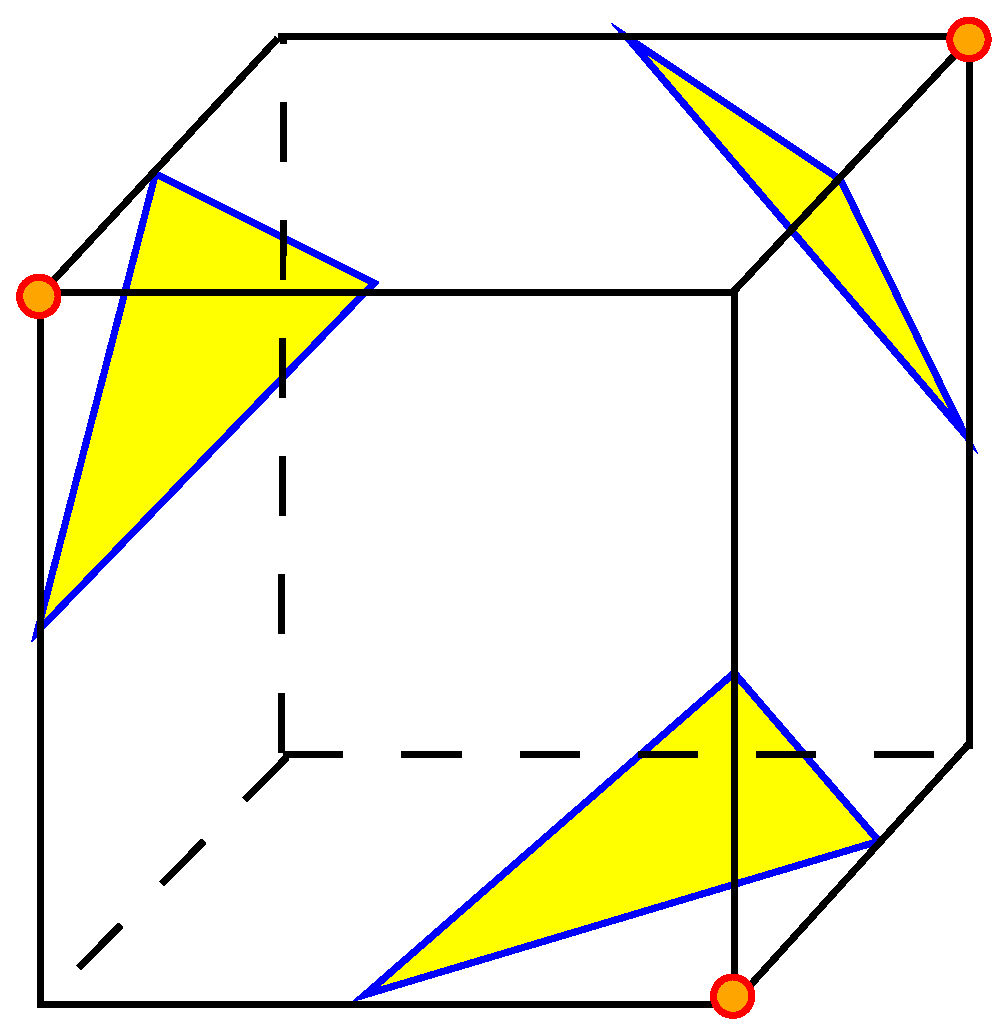
\includegraphics[scale=0.15]{../img/mar_cub_case7.eps}
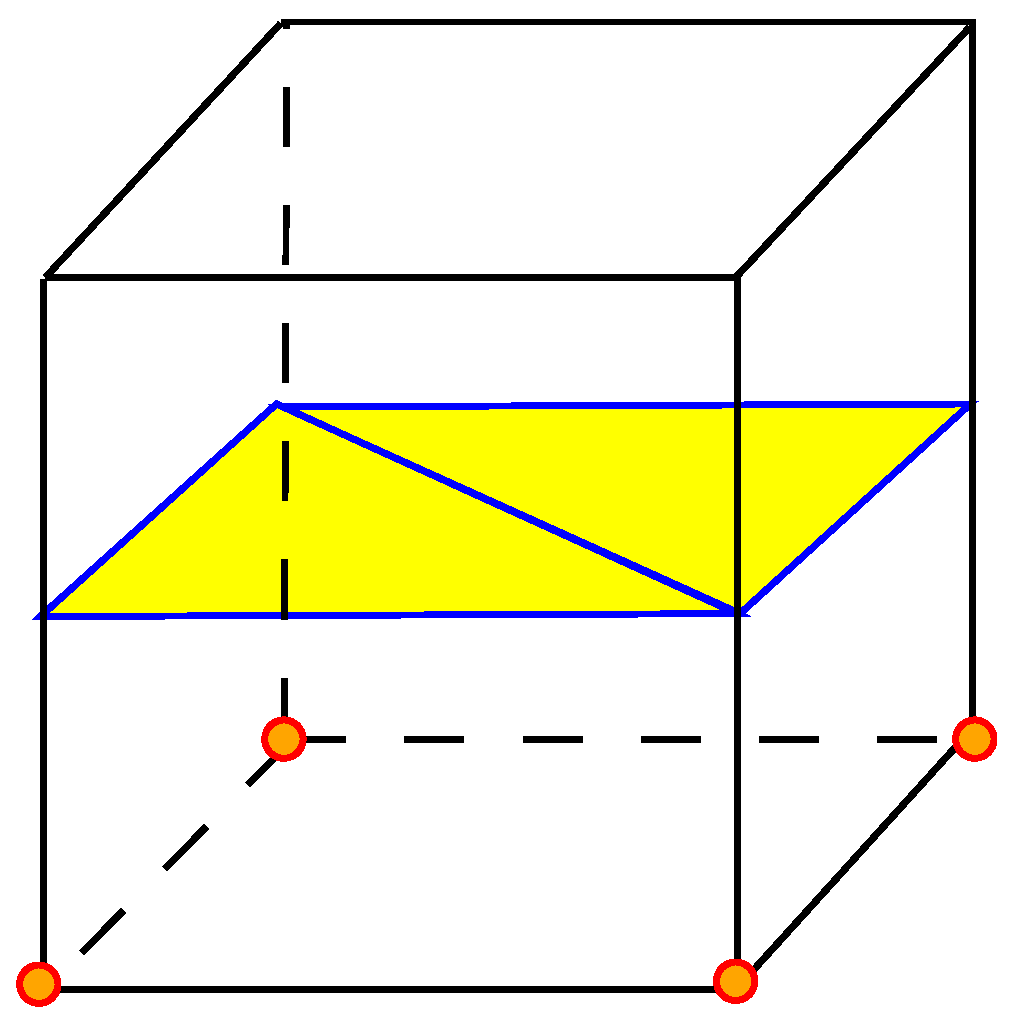
\includegraphics[scale=0.15]{../img/mar_cub_case8.eps}
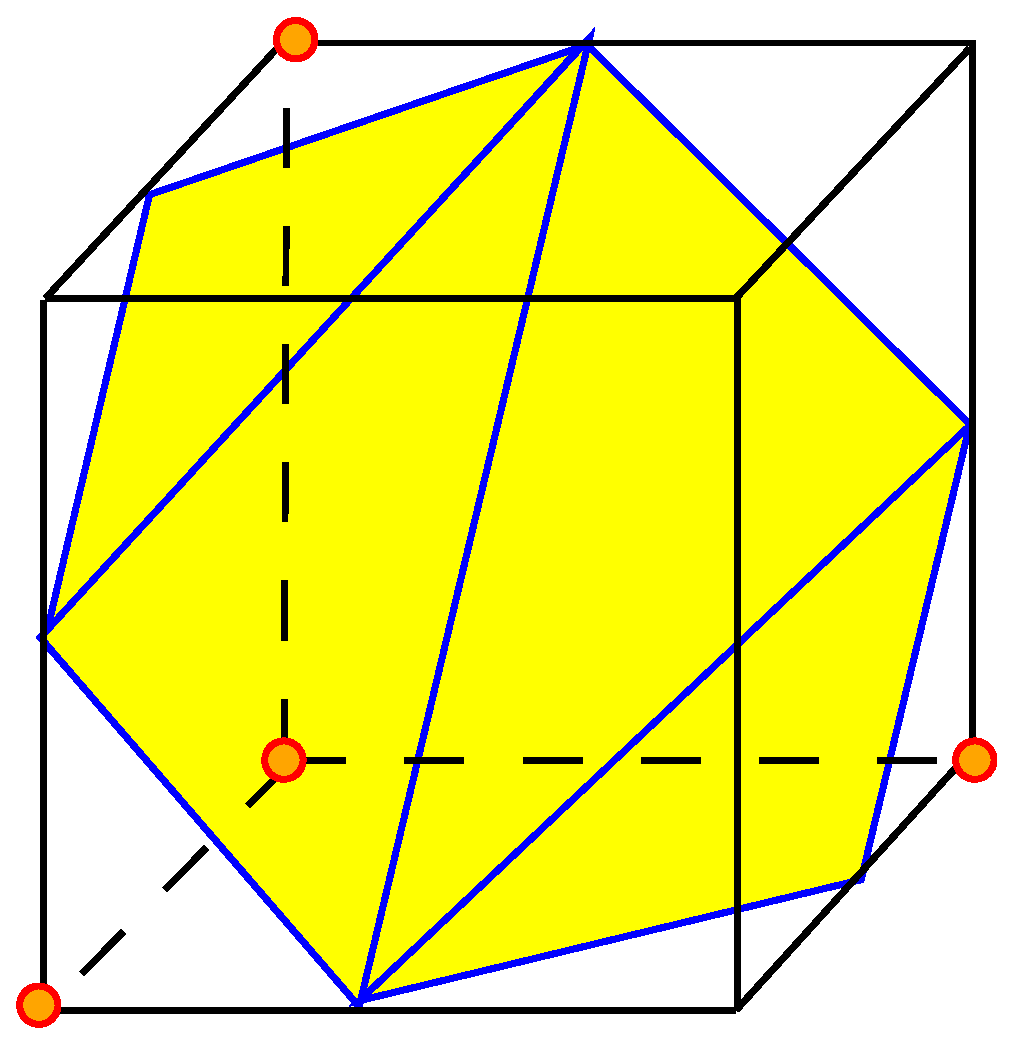
\includegraphics[scale=0.15]{../img/mar_cub_case9.eps}
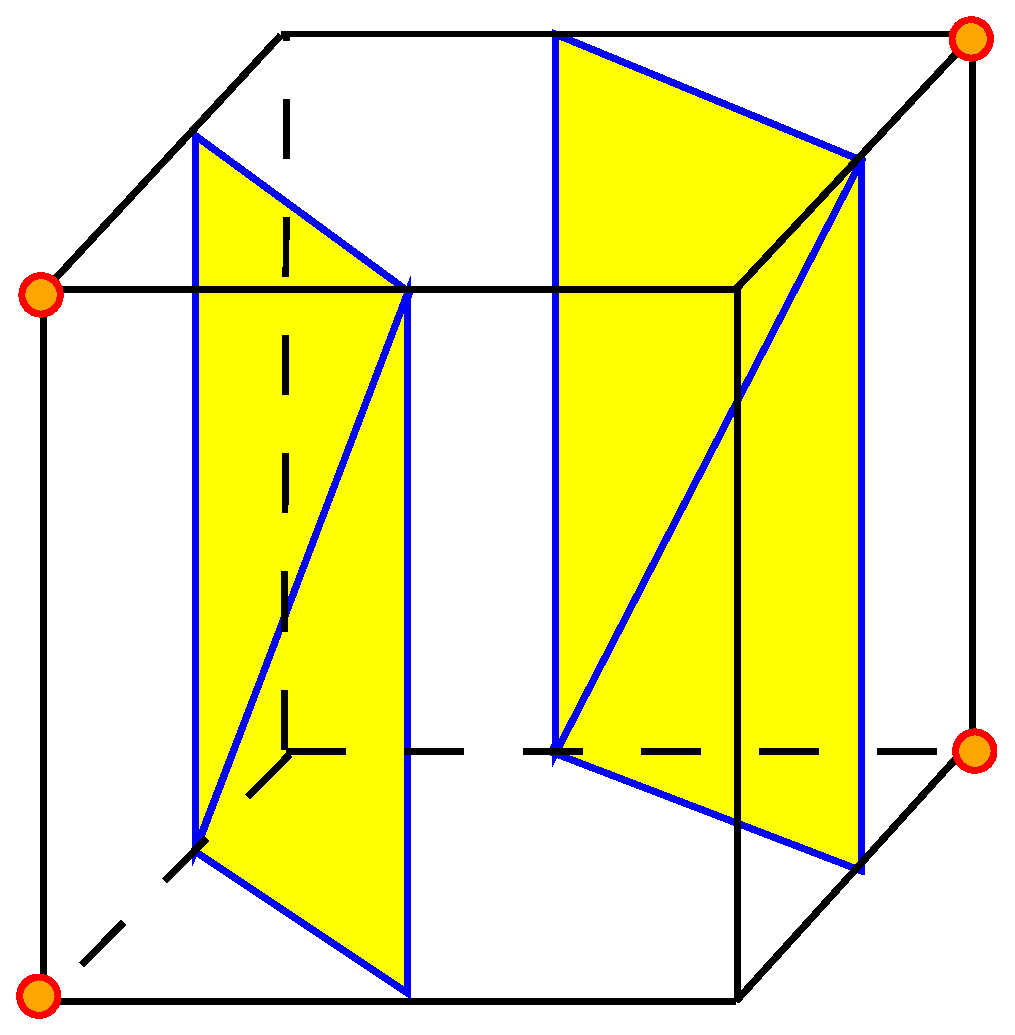
\includegraphics[scale=0.15]{../img/mar_cub_case10.eps}
\hspace{1mm}
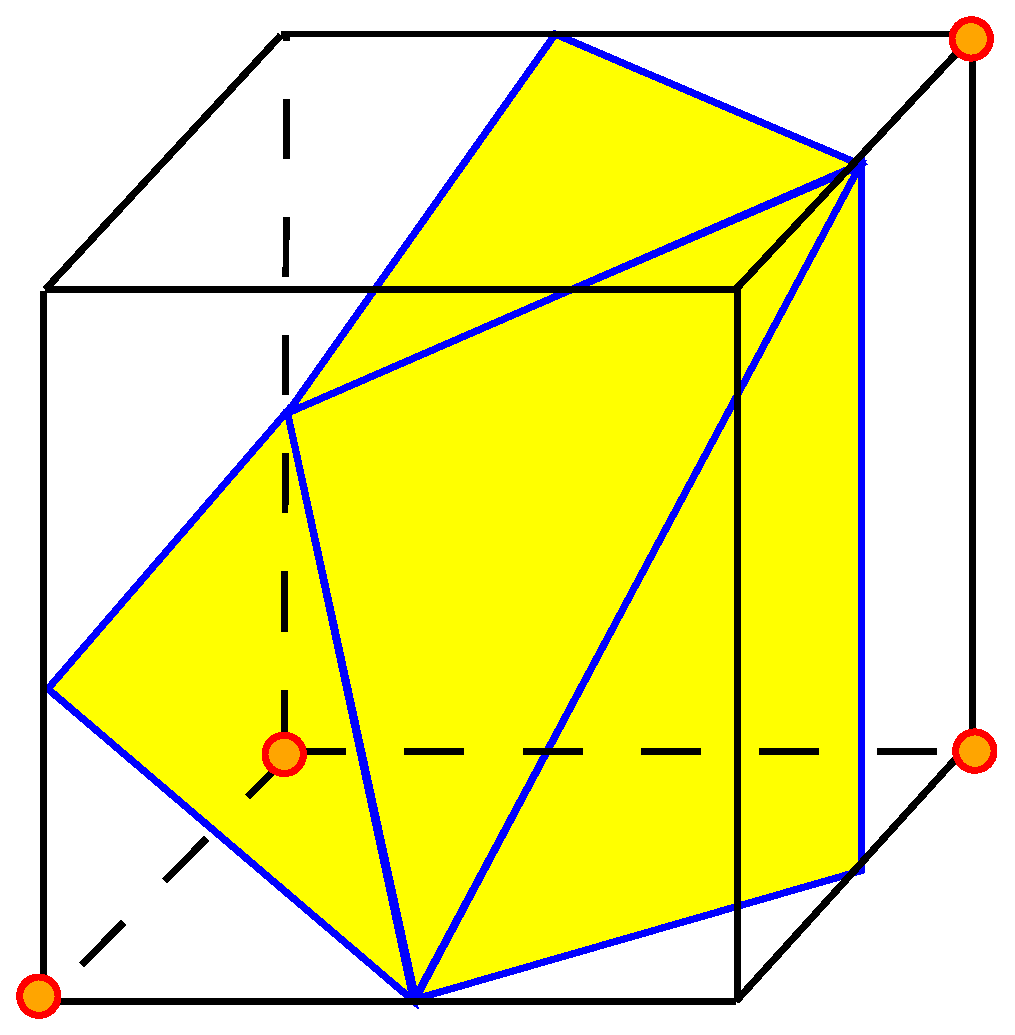
\includegraphics[scale=0.15]{../img/mar_cub_case11.eps}
\hspace{2mm}
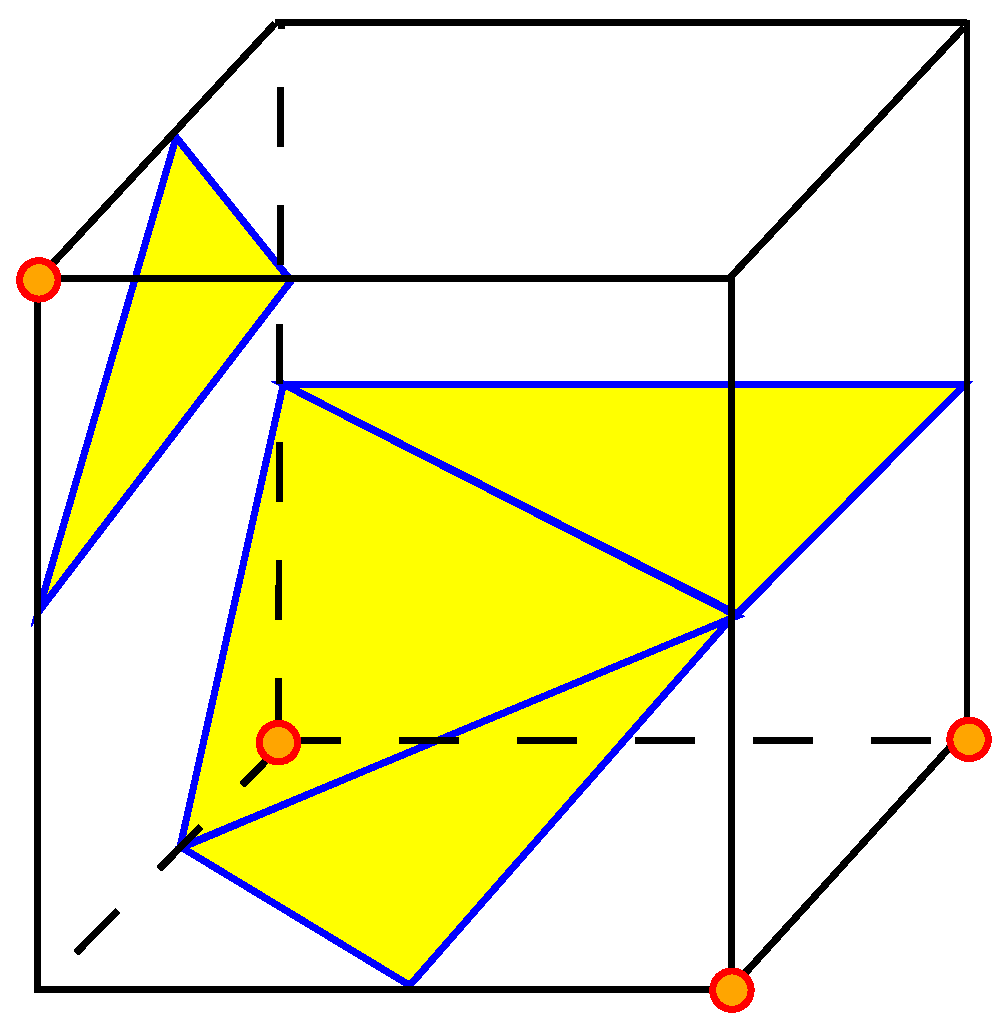
\includegraphics[scale=0.15]{../img/mar_cub_case12.eps}
\hspace{2mm}
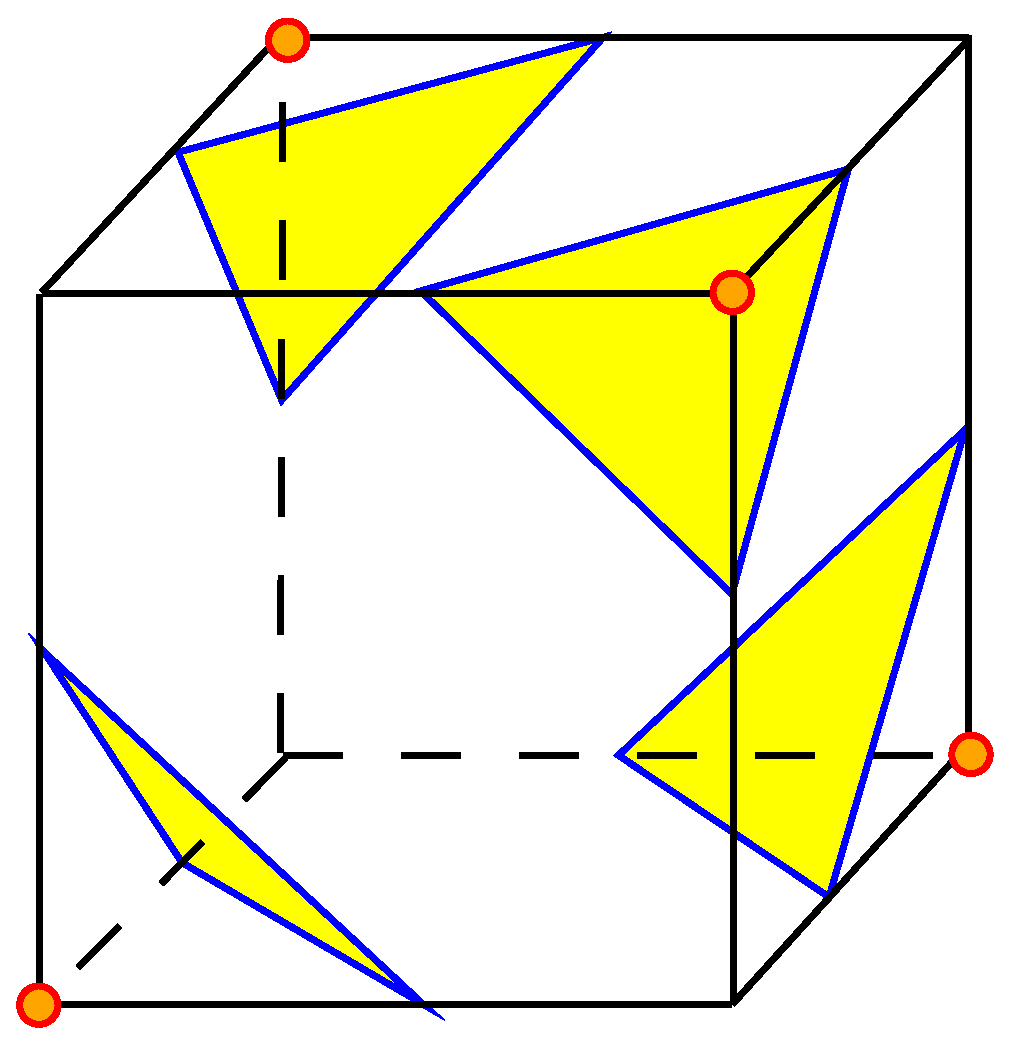
\includegraphics[scale=0.15]{../img/mar_cub_case13.eps}
\hspace{3mm}
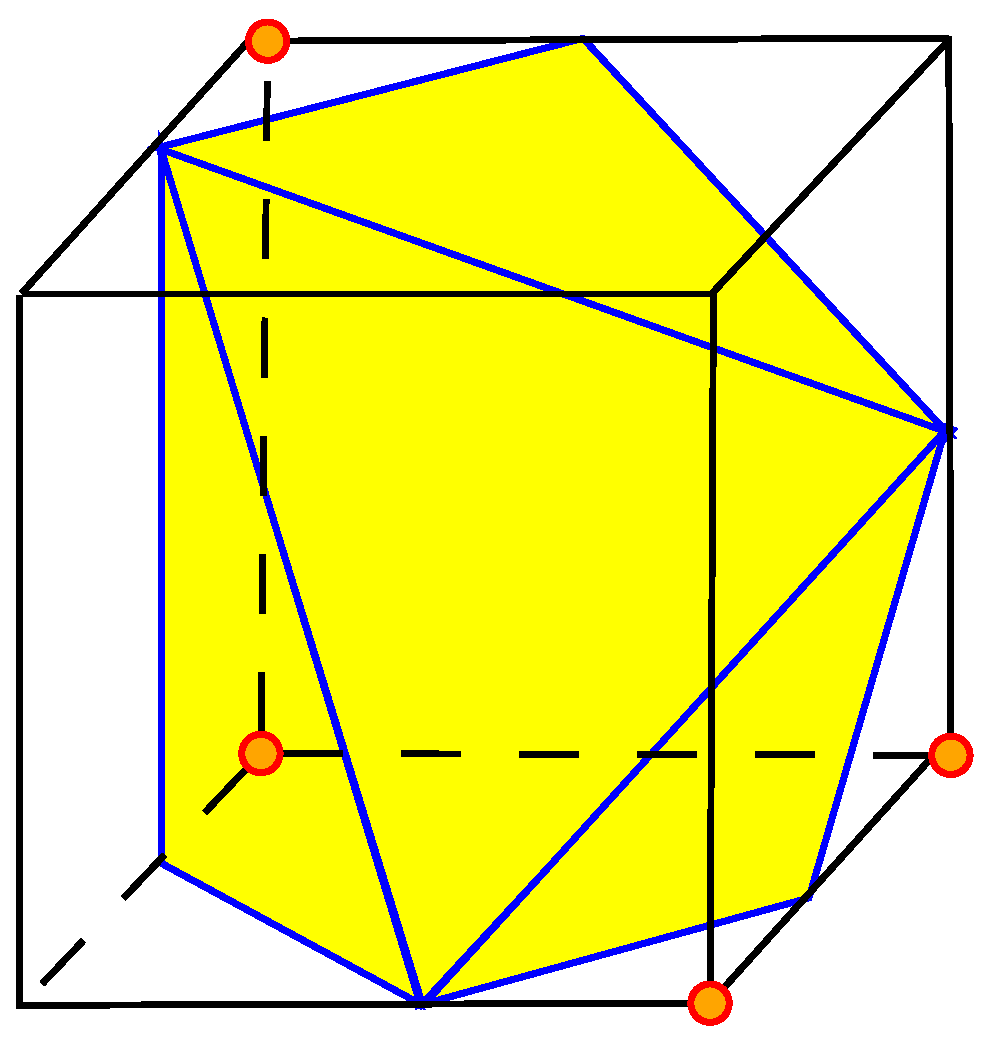
\includegraphics[scale=0.15]{../img/mar_cub_case14.eps}
\caption{The 15 cases of marching cubes algorithm. The corners that are evaluated as inside of the object
are labeled with red. The yellow triangles represent faces to be added to mesh.}
\label{fig:mc_cases}
\end{figure}

Finaly, all of them can be reduced to $15$ unique cases. The main idea of this algorithm is to
place a set of faces for each cube in order to create a polygonal mesh with a corresponding shape.
In the other words, each configuration refers to the configuration of new faces to be added to a mesh.
However we know two adjoining elements share 4 corners, resulting faces are continuous certainly.
If corners contain any other information except from inside/out information, the position of 
the faces in the mesh can be refined. Usually it contains the information about a color or
a distance from point to surface. In that case, placing or any other processing of
the face is based on linear interpolation corner values.\\
\\

\begin{figure}[!htbp]
\centering
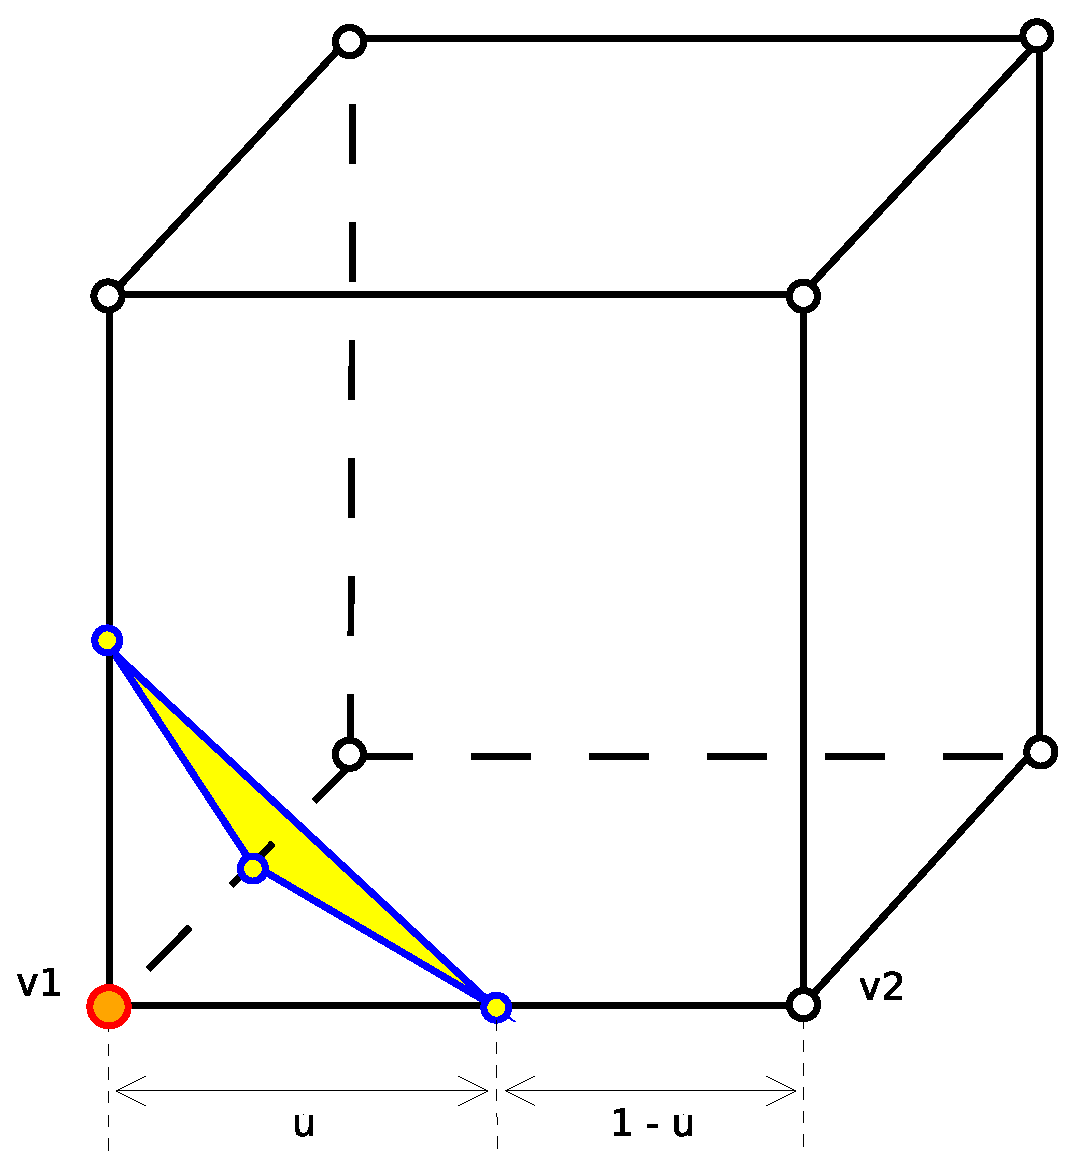
\includegraphics[scale=0.35]{../img/marc_cub_inter.eps}
\label{fig:mc_interpolation}
\caption{Interpolated position of face}
\end{figure}

Let $v1$ and $v2$ be the values that represents a distance from a surface to the corner.
Thus we can calculate the value of coefficient $u$ from following equation.

\begin{equation}
u = \frac{v1}{v1-v2}
\end{equation}

%This algorithm requires the capability of voxel map (or any other grid-aligned data structure) to
%determine corners configurations of arbitrary voxel (or proper element of representation). In the other
%hand, algorithm needs standard operations for creating faces and vertices of mesh.

\subsection{Voxelization}
\label{sub:vox}

In 2D, known as \emph{rasterization}. The algorithm that constructs an initially empty 3D grid and fill 
the
grid elements that indicates whether the element is inside the object. There is a several techniques
to represent a boundary element. The simpliest one is to set the boundary element as completely filled, 
thus we have a voxel map of values $0$ and $1$.\\

Algorithm can be divided to two phases: The first phase voxelizes the faces of triangle mesh and the
second one fill the created object. Admittedly, before the filling the object algorithm has to check,
whether the mesh forms an enclosed surface. If it does not form an enclosed surface, the second phase of
algorithm is omitted.\\

First phase voxelizes faces one by one. Each face is processed similarly like in the triangle 
rasterization in 2D.
First, algorithm voxelizes the boundary edges and then runs floodfill over the face. The filling
technique of the face is is processed by the line filling algorithm in following steps. 

\begin{figure}
\centering
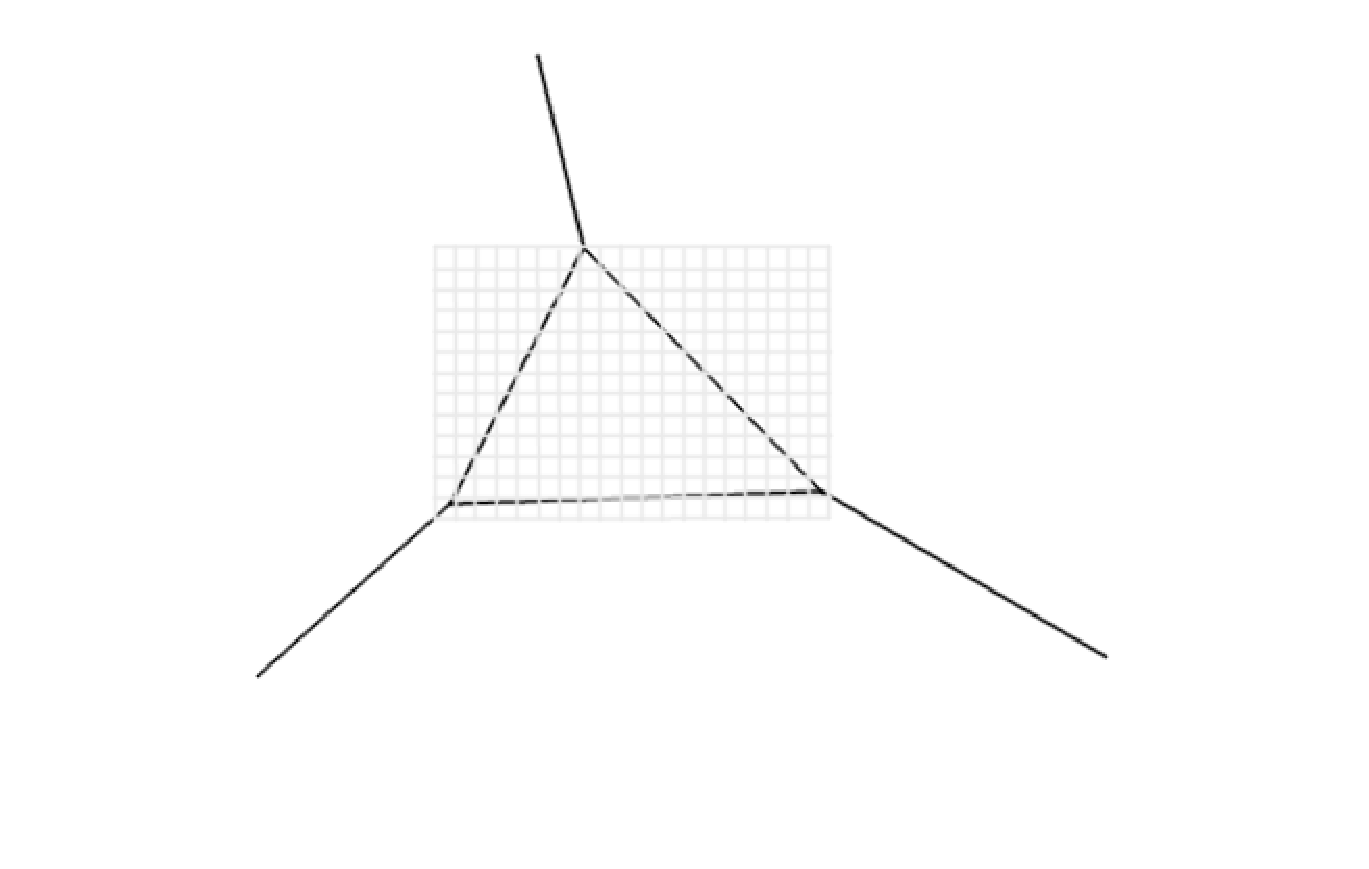
\includegraphics[scale=0.25]{../img/voxelize_1.eps}
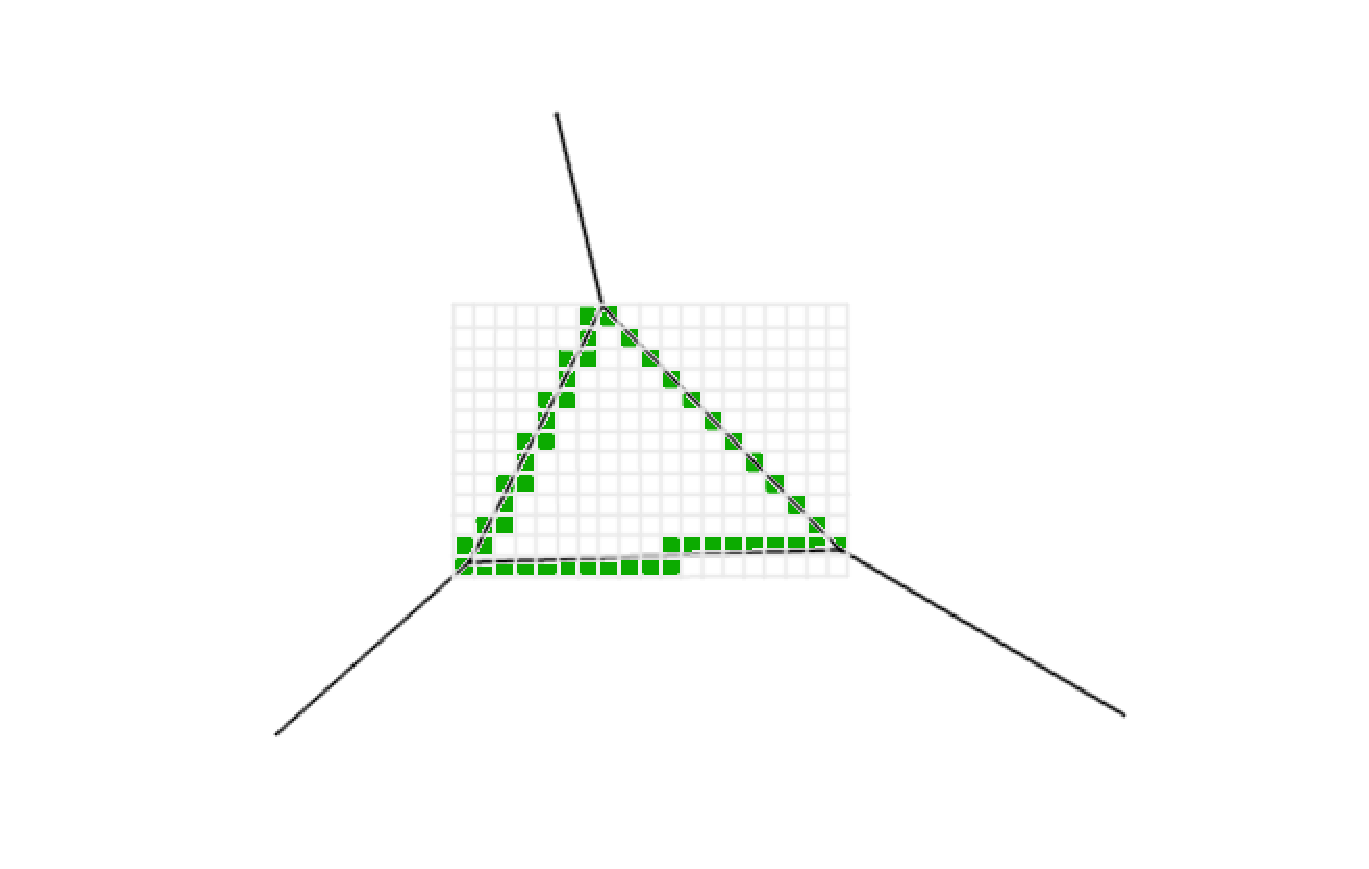
\includegraphics[scale=0.25]{../img/voxelize_2.eps}\\
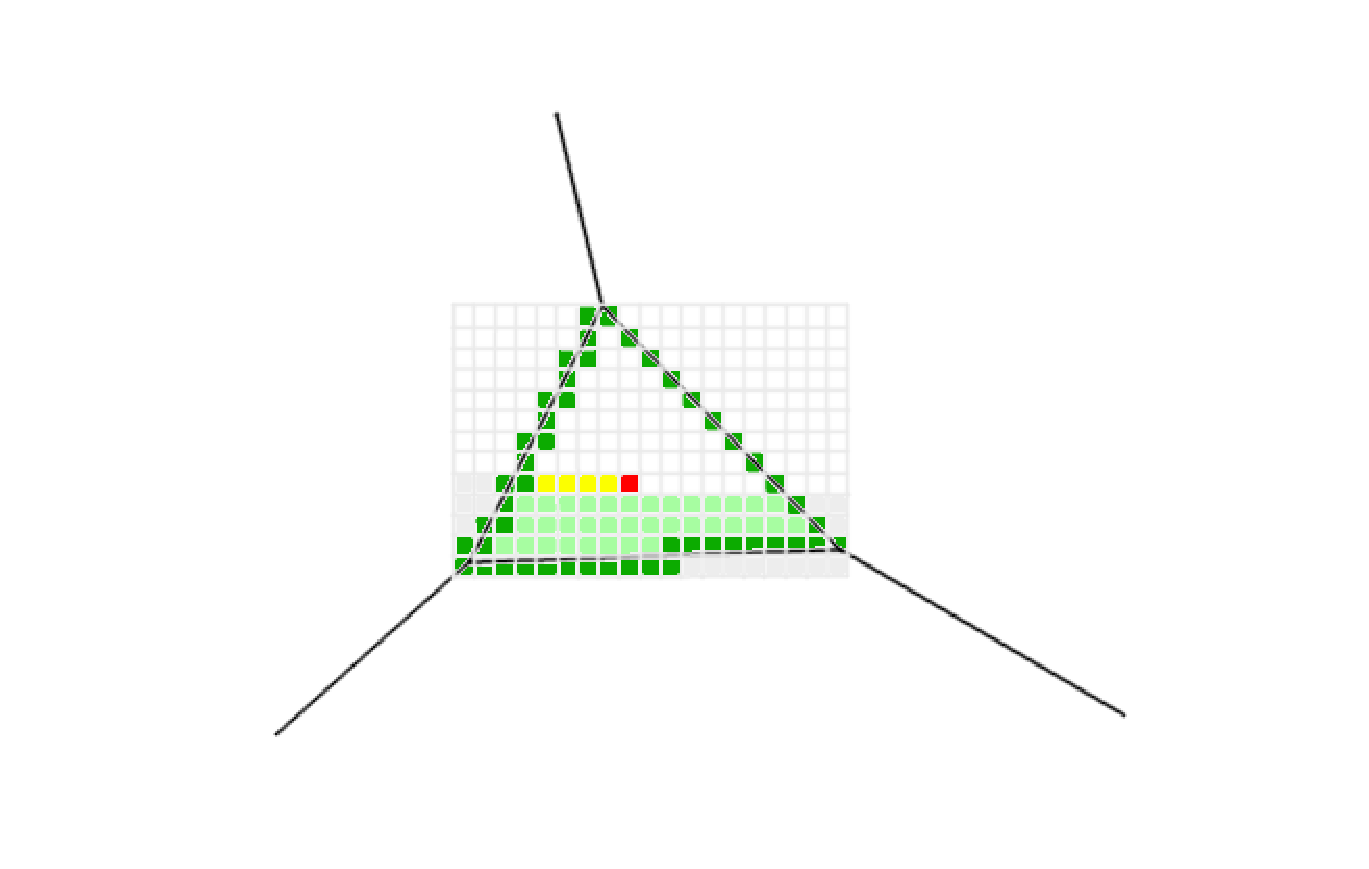
\includegraphics[scale=0.25]{../img/voxelize_3.eps}
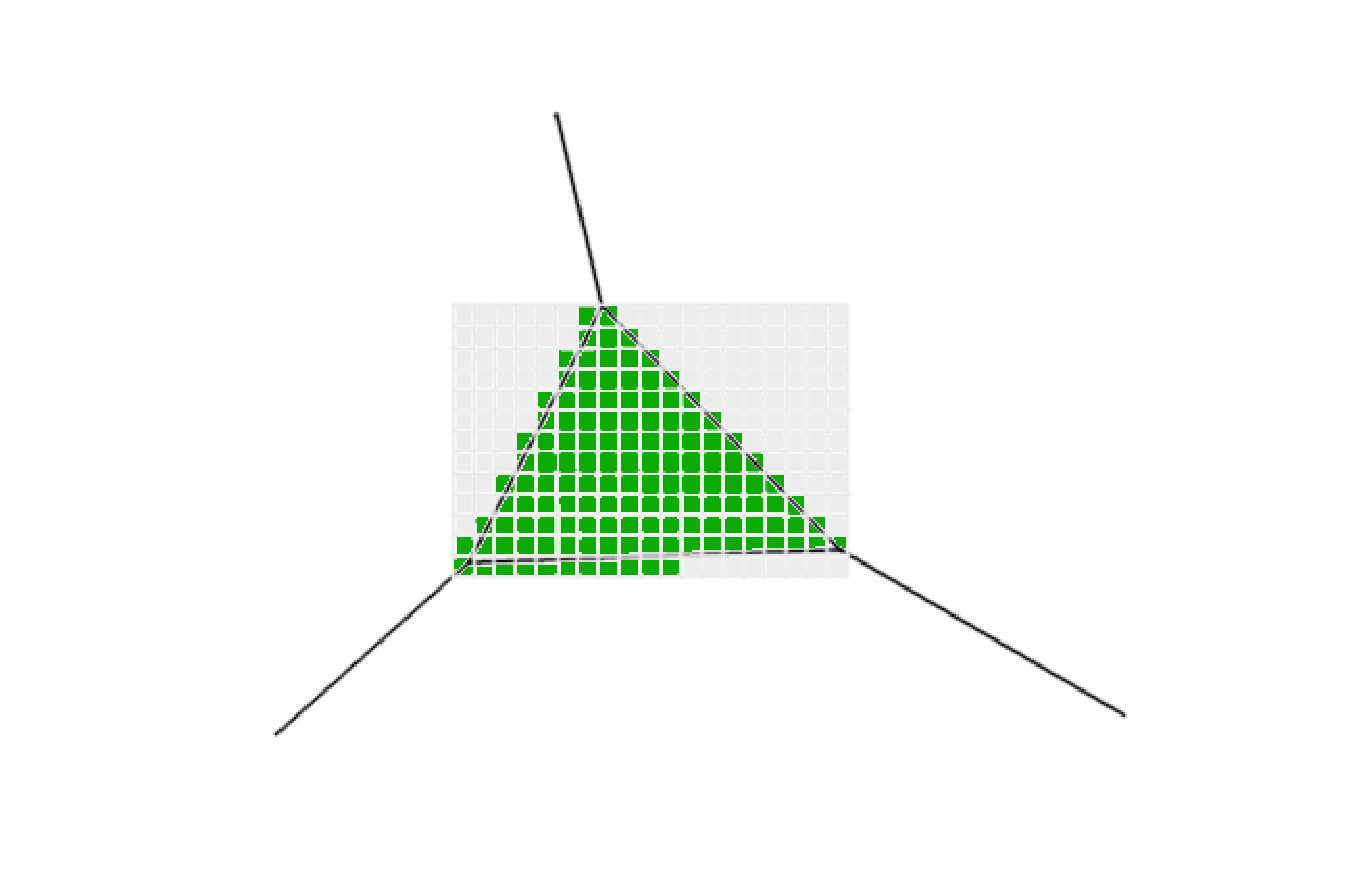
\includegraphics[scale=0.25]{../img/voxelize_4.eps}

\caption{Voxelization in step-by-step}
\label{fig:voxelize}

\end{figure}

\begin{itemize}
\item On the pre-computed minimum boundary rectangle start on the bottom and repeat for each line
\item in the line start from arbitrary side and process the elements consequently
\item After first crossing a rasterized edge start filling the elements (entry the face)
\item After second crossing a rasterized edge stop filling (leave the face).

\end{itemize}

In the second phase the algorithm fills the elements inside the object. The only problem is to
determine whether the given voxel is inside or outside the object. As described above, assumption of
starting with line outside the enclosed area gives us the right method. Also in this case the
bounding box will be needed. If the object cannot be wrapped the inside/outside property of element can 
not be determined.

\section{Editing functions}

Some functions are designed to changing size or shape of the object. Those functions are called 
\emph{editing function}.
During the editation of the object, user defines required values and the function deforms the
object properly. In case of the editing function \emph{scaling} for instance, a user defines the scaling
ratio.

\subsection{Truncate}

Truncate is the operation that affects a topology of mesh. From a given vertex it creates a new face with
surroundings of the original vertex. This is a common operation of mesh editation used e.g. in
3D editors.\\

\begin{figure}[ht]
\centering
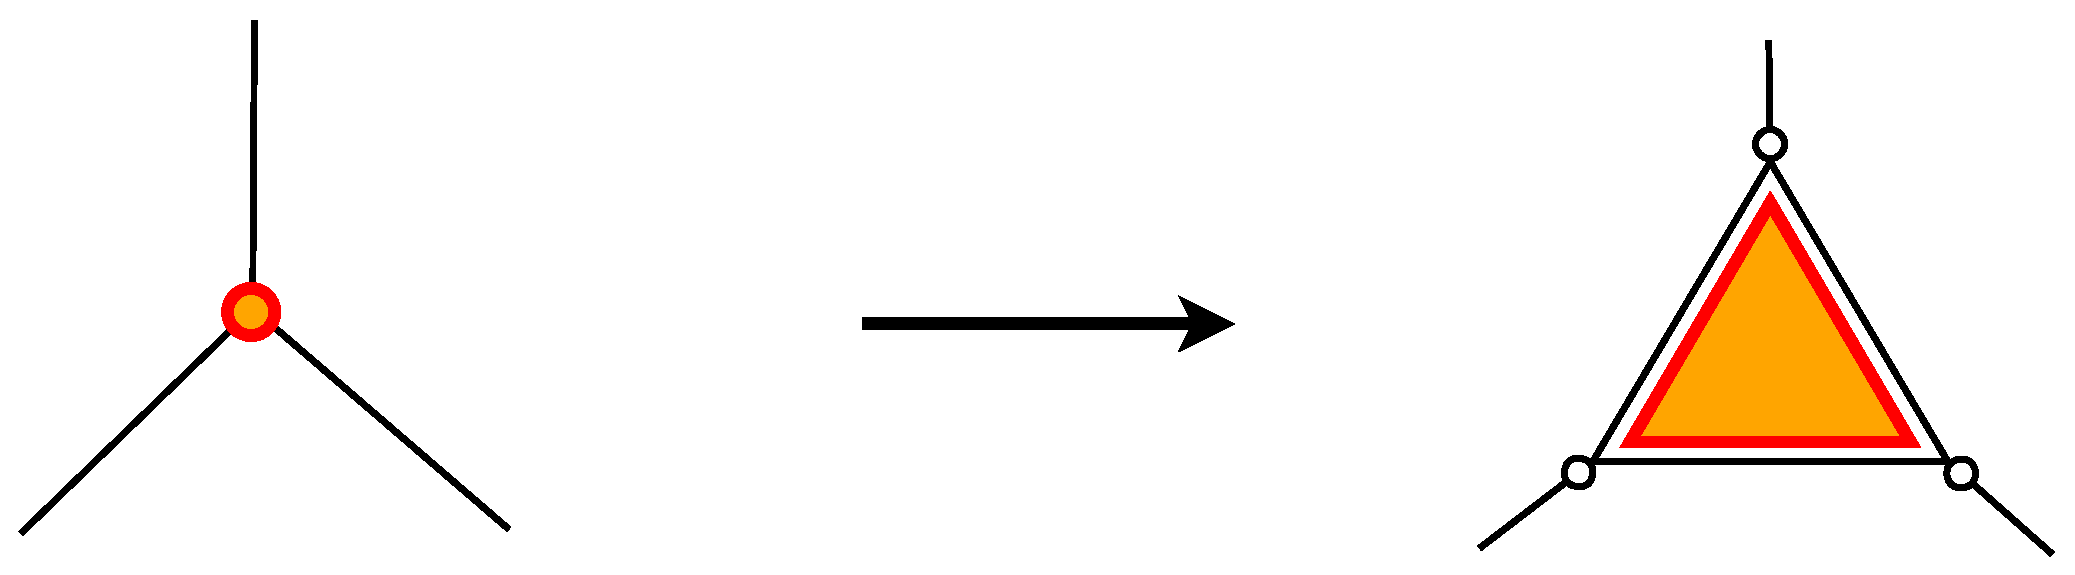
\includegraphics[scale=0.2]{../img/truncate.eps}
\caption{The red-marked vertex is a selected vertex to be truncated.
The face filled by orange color with red borders is the resulting face created by truncation}
\end{figure}

%This algorithm requires the capability of mesh to query the surrounding vertices of given vertex and
%adding the vertices and faces to the mesh.

\subsection{Bevel}

This operation is almost identical with \emph{truncation}. The only difference is the argument of the
operation. As the truncate operation creates a new face based on the given vertex, the bevel operation
creates the face from a given edge.\\

\begin{figure}[ht]
\centering
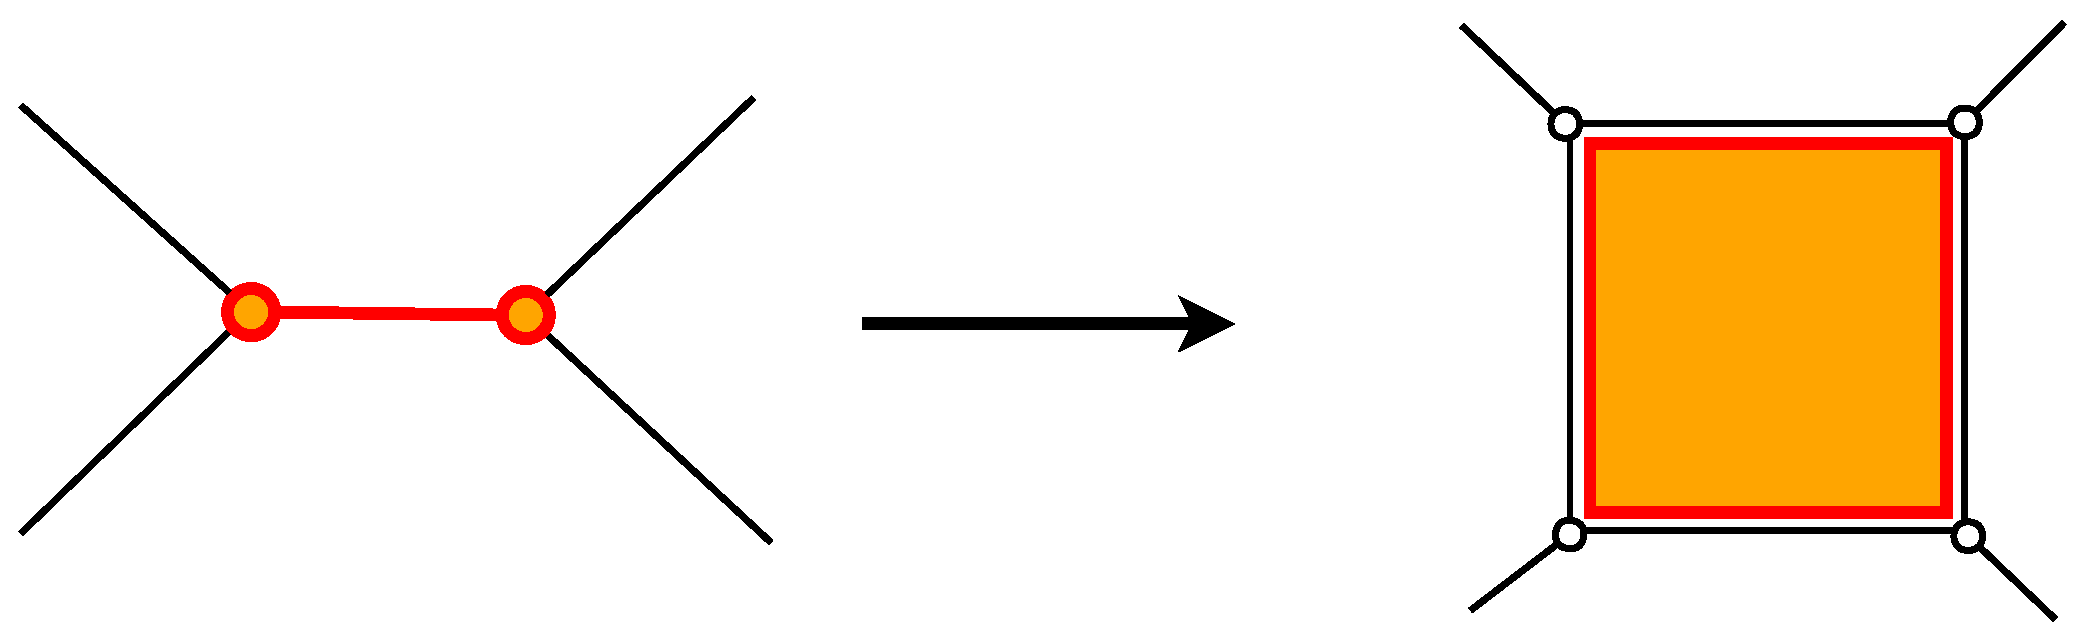
\includegraphics[scale=0.2]{../img/bevel.eps}
\caption{The red-marked edge is a selected edge to be beveled. As in the previous case, the resulting
face is filled by orange color.}
\end{figure}

%This algorithm has the same requirements as the truncate. In addition it requires the capability of
%querying to surrounding vertices of given edge.

